\documentclass[11pt]{article}
\usepackage[top=1.00in, bottom=1.0in, left=1in, right=1in]{geometry}
\renewcommand{\baselinestretch}{1.1}
\usepackage{graphicx}
\usepackage{natbib}
\usepackage{amsmath}
\usepackage{multicol}
\usepackage{tcolorbox}
\usepackage{caption}

\bibliographystyle{besjournals}

\begin{document}

\title{Closing the gap between statistical and scientific workflows for improved forecasts in ecology } 
\date{\today}
\author{Victor Van der Meersch, J. Regetz, T. J. Davies$^*$ \& EM Wolkovich}
\maketitle
$^*$ Says he is happy to help and give friendly review, but not sure he will reach level of co-author. 

{\bf Deadline:} 1 May 2025 (was 1 April 2025)

\emph{For:} Scientific and Statistical Workflow theme issue for \emph{Phil Trans A} as an \emph{Opinion}
% They mention a tex template here: https://royalsocietypublishing.org/rsta/for-authors#question4
% Word length: I should check what they emailed but they say no more than 13 printed pages with 650 per page (whoa, we should be well below that! I am thinking 3-5K would be good)
% Already 5K! 

% To do:
% Fix the abstract so it matches the paper better (I think mainly the last few sentences need work, or we just need to say more about data sharing in the text)
% Add in Figures
% Delete out unnecessary comments so easier for co-authors to read?

\begin{abstract}
Increasing biodiversity loss and climate change have led to greater demands for useful ecological models and forecasts. Relevant datasets to meet these demands have also increased in size and complexity, including in their geographical, temporal and phylogenetic scales. While new research often suggests that accounting for these complexities variously increases, removes or otherwise alters major trends, we argue that the fundamental approach to model fitting in ecology makes it impossible to evaluate and compare models. These problems stem in part from continuing gaps between statistical workflows---where the data processing and model development are often addressed separately from the ecological question and aim---and scientific workflows, where all steps are integrated. Yet, as ecologists become increasingly computational the opportunity to close this gap has never been greater. We outline how increased data simulation at multiple steps in the scientific workflow could revolutionize our understanding of ecological systems, yielding new insights for both trend estimation and forecasting.
%Combining these changes with more open model and data sharing---and developing new efforts to race the same data---could be transformative for ecological forecasting. 
A shift toward universal training in a more robust model building could bridge the gap between process-based and statistical approaches and be transformative for ecological modeling.
\end{abstract}

{\noindent \bf Goal:} Increase awareness of how we can merge statistical and scientific workflows in ecology (especially forecasting) and what we would get out of it.
\vspace*{0.5cm}

\section{Introduction}

Anthropogenic drivers are reshaping natural systems, with impacts expected to increase in coming decades \citep{Diaz2019}. Climate change will likely accelerate biodiversity loss, altering ecosystem services and human well-being \citep{IPBES2019}. Implementing sustainable policies to mitigate these impacts is thus a global priority, but designing the best policies requires estimating and understanding biodiversity and ecosystem trends to date alongside the skill to forecast future dynamics. % These requirements in turn have created a growing need for more global ecological data, and the types of models that can robustly handle such data. 

Meeting these policy needs has led often to two separate paths: one focused on estimating trends from new global datasets and another focused on forecasting from generally distinct datasets or mechanistic models based on less data. Newly available large-scale, long-term datasets have provided our first `global' estimates of biodiversity trends \citep[e.g.][]{Dornelas2018}, but these data---gathered opportunistically from multiple sources---are unbalanced with massive geographic, temporal and taxonomic biases. Models to date have failed to fully address these challenges and, perhaps because of these limitations, are rarely if ever used for forecasting. 
Instead forecasting---under different plausible scenarios---has generally relied on entirely different datasets combined with either correlative or process-based models \citep{IPBES2019}, with process-based models often promoted as the most realistic approach \citep{Urban2016, Pilowsky2022} because they focus on mechanistic representations of ecosystem functioning. The current outcome from these approaches is no clear agreement on current species trends, with ongoing debates on the magnitude and even direction \citep{Dornelas2014, Leung2020, Buschke2021, Johnson2024}, and forecasts that diverge due to high model uncertainty at the ecological level \citep{Cheaib2012}. 

We argue that current debates and diverging forecasts are driven in large part by the incoherent and disconnected workflows used today in ecology \citep{Loreau2022, Talis2023, Johnson2024}. Research estimating biodiversity trends has become focused on methodological aspects because the current workflow fails to examine the gap between ideal and available data, and rarely tests for predictive accuracy that could scale up to allow forecasting. At the same time, forecasting-focused process-based models often develop by adding a new separate layer, disconnected from the original research aim, the data stream and the previous scientific insights, because they fail to examine the model as a functioning whole and thus ignore major degeneracies. 

Workflows that fully integrate all the steps required to build a model from an ecological question, evaluate its limitations and degeneracies, before estimating its parameters and making projections, could reduce many of these problems. In particular, we argue that workflows that incorporate data simulation at multiple steps can quickly identify flaws in model structure and constraints in data. Towards this aim, here we outline the steps of a universal workflow that could harmonize both trend estimation and forecasting.

\section{Scientific method and workflows}

Quantitative science relies on a model-based framework, to confront hypothesis and data \citep{}. In an idealized scientific method, we would formulate a research question and hypotheses, design an experiment accordingly, build a model, collect data, and using this data to inform our model and differentiate between hypotheses. But this idealized method often does not apply to the reality of ecological research. Many important questions cannot be addressed through controlled experiments and replications. Instead, we must often rely on existing, heterogeneous datasets alongside uncertain and incomplete theory to provide a large-scale and long-term perspective \citep{Hilborn1997}.

This reality should drive researchers to use more robust and coherent methods, but the current workflows combined with the challenges ecologists are facing instead appear to be leading to persistent problems. 
Trend estimation has focused mostly on fitting the model to empirical data in a uni-directional way that makes feedbacks to highlight uncertainty and related limitations in the model and/or data rare (Fig. 1). For forecasting, researchers focus on making predictions with increasingly complex models, making the steps for model building and parameterization increasingly obscured (Fig. 1). Today, researchers often calibrate different parts of the model separately, and fix some parameter values based on experiments and expert knowledge, to avoid problems when trying to fit the model as a whole. Addressing these problems while accounting for the realities of working with ecological data requires a more comprehensive workflow. 
% mention the disconnection between trends and forecasts?

\begin{figure}[h]
	\centering
	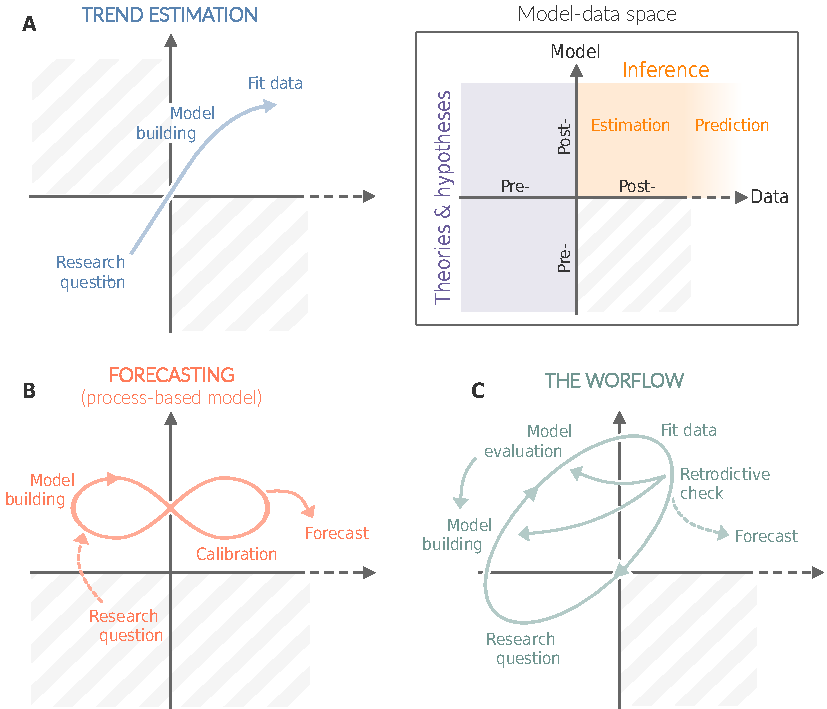
\includegraphics{figures/modeldataspaces}
	\caption{} 
	\label{fig:modeldata}
\end{figure}

We argue a workflow that moves along the data-model space in a coherent sequence of steps with repeated data simulation (Fig 1) could reduce many of these problems and thus improve ecological science.
The first step of the workflow is to define an explicit research question and formulate hypotheses (Fig 2). This involves making clear assumptions about the most influential drivers, within the specific context of our study. This step help us to think about the mechanisms that could generate the data we observe, including the observational error. Naturally, this leads to the development of a model---an ensemble of mathematical equations that encapsulates our knowledge and designed to answer our research question. The general idea is to start with a relatively simple model, that we could refine later. At this stage, prioritizing biologically meaningful parameters is crucial, as it allows us to have a sense of plausible parameter values. 

With a model in place the next step focuses on testing and understanding it via data simulation. `Fake' or `test' data are generated directly from the model by fixing parameters to some values (which is straightforward if the parameters are interpretable) and from fake predictor data. This simulated data should reflect the full model assumptions, and could begin to include complexities in our data structure and biases, which may in turn lead to adjusting the model. For example, if a researcher realizes their empirical is geographically biased, that should be built into the model and thus then into this data simulation step. 
We then fit our model to this simulated dataset and evaluate its ability to recover the prescribed values. 
Once we are confident about our model structure, we can incorporate real data. This way, we obtain parameter estimates constrained by observations. Here, difficulty in fitting the model might indicate an inherent need for more data to address our initial question. This could lead us to either simplify our research question or---ideally---launch new data collection efforts. This leads to the second data simulation step, this time using our fitted model parameters to generate predictions. This retrodictive check allows model output to be compared to observations. 
The workflow replaces parameters at the core of the modeling process, as fundamental components that shape both inference and forecasting. Any parameter (such as a trend estimate) must be carefully interpreted alongside others. %such as the  global mean or intercept and the estimate variance
Within such a workflow, forecasting emerges as a natural outcome: rather than being a final goal, it only involves jointly modeling new circumstances along with the original data.

\begin{figure}[h]
	\centering
    \hspace*{-1.5cm}
	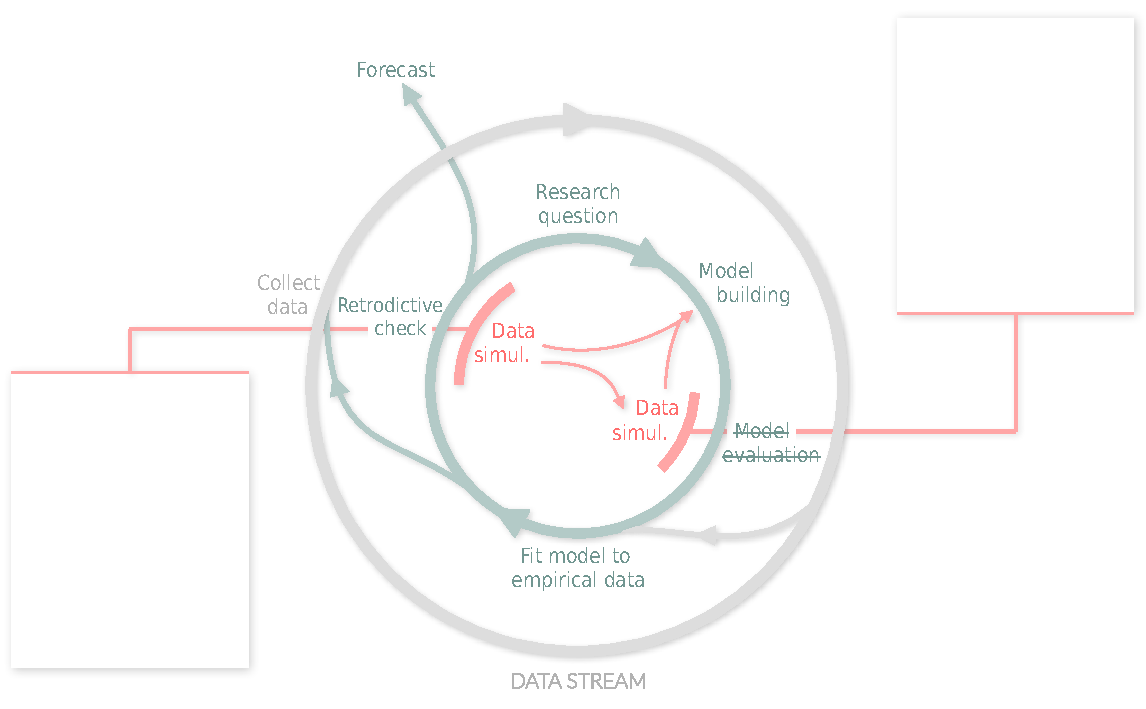
\includegraphics{figures/figure_worflow}
	\caption{} 
	\label{fig:modeldata}
\end{figure}

% More details, what's special! Feedbacks!
%emw6Apr: I think there's more than just degeneracy here, often people build in more complexity to their simulated data than their model allows, but this means they should change the model (or the question). This needs to be clearer above and below. I think this is the first point (since it's a little more obvious to readers and it relates to trends, which we always handle first), and the next one could be about structural degeneracies  but I think we need to be careful here in what we mean and explain it more to readers who will not get it. 
A key feature of this workflow is the central role of data simulation, which introduces two feedback loops. The first feedback arises when we evaluate the model on simulated data.
The failure of the model to recover known parameter values and handle the complexity of the simulated data should prompt a reconsideration of the model, or even a reformulation of the research question.
Further, % structural degeneracies in the model might become apparent, 
this step might reveal that some parameters are highly non-identifiable,
flagging % not sure about this word
the need to change the model structure---before incorporating real observations. 
The second feedback loop comes from the retrodictive check. 
Discrepancies may indicate a missing key driver---perhaps an expected outcome if we known our initial model was too simplistic. We can refine the model to integrate the missing process and restart the workflow. Insights from the retrodictive check can also lead us to introduce additional complexity when simulating fake data, such as phylogenetic structure or observational biases (e.g. unbalanced data). This iterative evaluation of the model moves beyond a simple reliance on goodness-of-fit metrics. At each iteration, we are able to evaluate the model behavior, both with simulated and real data, taking into account our expert knowledge of the ecological processes. 

\section{The workflow in practice}

%emw6Apr: I like the shift to 'parameter estimation' instead of trend estimation, but I wonder if we could make that shift clearer above. Maybe somewhere we say that the workflow would  encourage a focus on the full model and its parameters: For trend estimates, the trend becomes just one parameter that must be carefully interpreted alongside others . 
Across the different fields of ecology---for both parameter estimation and forecasting---a systematic application of a coherent workflow could highlight the best opportunities to reduce uncertainties through new scientific insights, toward the most critical steps. This will help refocus the debate on designing new hypothesis, formulating new questions---and guiding efforts to collect new data. Here, we illustrate how such a workflow could lead to significant improvements in two case studies: (i) estimating global biodiversity trends and (ii) forecasting future species and ecosystem dynamics using process-based models.

\subsection{Trends}

Ecologists have now amassed data on populations and species over the globe, they have also engaged in an increasing number of debates on regional and global trends, with arguments over the magnitude and even direction \citep{Dornelas2014,Leung2020,terry2022no,muller2024weather}. Apparently conflicting results have made it harder for policy-makers to advance initiatives aimed at slowing declines, and has led to a debates within ecology about whether such analyses undermine public confidence in science  \citep{gonzalez2016estimating}. While shifting estimates are part of the process of science---refining our approaches and thus estimates over time---we argue much of the work underlying these debates stems from a poor workflow. 

An improved workflow that required retrodictive checks and data simulation would lead to larger model advances and a greater recognition of uncertainty---thus highlighting likely consistency in estimates across models---that could better aid policy.  Using the workflow would make what now appear as major discrepancies more obviously shifts in point estimates that are generally all in the same uncertainty space \citep{Johnson2024}---and it would challenge modelers to show major predictive advances, which is not currently part of the process. Explanatory power in most models of observational data is usually very low \citep{low2014rising,moller2002much} and thus tests of models' predictions rarely expected. But the workflow highlights that predictions from the model---what we call retrodictive checks (or whatever we call them)---are part of the process of science, and critical to testing for what may be missing in a model. We expect retrodictive checks on most published trend analyses would highlight major missing components in these models (expand here?? ADD example?), and drive changes both in the models themselves and in the simulated data to check the models. While ecologists have started to use simulated data more to understand potential limitations of their models and data combined, this is still extremely rare, and efforts to date often treat simulations as separate from the statistical model \citep{Buschke2021,dove2023quantifying}, short-circuiting their full utility
% Mention how low R2 are in ecology?
% Simulating data to verify and test models in trend analyses is currently rarely reported, which we believe makes it easier for ecologists to fit poor models and in turn debate them.. 
% Mention elephants rebounding...

% Trends - improvements!
Applying the workflow to current trend estimates could importantly highlight the best way to improve data collection for more reliable estimates. Returning to the example of a global estimate of trends in vertebrate populations of species over time and applying our proposed workflow would mean more efforts to define the goal and question---is it a simple global estimate? Or a need to also find which species are declining most, including those that may have poor or no data? From there a generative model using simulated data for testing could incorporate many aspects of the populations, and data, that are often only included in `null' or 'synthetic data generation' currently \citep{Buschke2021,mcrae2025utility} but could be built into the models fit to the empirical data. Eventually fitting the empirical data and performing retrodictive checks would likely highlight major missing components of the generative model. For example, certain populations are recovering for very specific reasons (e.g., elephants in regions where the ivory trade drove declines in the past) that perhaps should be modeled. From this model, what data are most critically needed to address the updated aims would become clearer and could drive new data collection \citep{toszogyova2024mathematical}. 

\subsection{Forecasting}

% vvdm07april: need to work on a better intro paragraph
Ecological forecasting is a broad field with a diverse range of methods. Process-based modeling is often considered the gold standard in ecology \citep{Urban2016, Pilowsky2022} and beyond. Newer models generally incorporate greater complexity and an ever-growing number of parameters, making it more difficult to increase scientific understanding \citep{Franklin2020}, and suggest or model potential policies. 

% vvdm07april: need a topic sentence
Increasing model complexity has not necessarily led to reduced uncertainty. In climate modeling, the uncertainty range on the effect of increasing CO2 concentration on temperature have remained largely unchanged \citep{Zelinka2020}. This has driven calls for more rigorous and transparent calibration processes \citep{balaji2022general}. Similar concerns arise in ecology, where strong disagreements exist about the effect of climate change on future species distributions \citep{Cheaib2012} and ecosystem dynamics \citep{Lovenduski2017}.
These uncertainties have large implications beyond ecology, as they influence simulations of biosphere-atmosphere interactions and, ultimately, future climate projections \citep{Bonan2018, simpson2025confronting}.
Some researchers now advocate for the simplification of models, to avoid over-parametrization when the data provide little information to constrain some parameters \citep{Wang2017, Harrison2021}. If a model becomes too complex, understanding the sources of uncertainty and how they propagate through the model may become nearly impossible.
Each additional process and parameter can increase overall uncertainty to the point where model projections lose their usefulness for decision makers \citep{Saltelli2020}.

Applying the workflow to process-based models is a key for opening the black box. It would serve as a guide through the successive steps of model development. In particular, incorporating data simulation would introduce a crucial step between model building and data fitting, ensuring a clear delineation between the two and exposing strong degeneracies in the model design. This approach would force researchers to begin with a simpler version of the model, providing a clear pathway to support---or reject---the additional complexity and new parameters along the iterative development of the model. 
Model calibration would no longer be just a hidden aspect of model building but a step as crucial as forecasting to gain new ecological insights. It would help properly take into account any issues regarding non-identifiability. This could involve reformulating the mathematical structure of some processes, making new hypotheses to target the right level of complexity, or incorporating more expert knowledge to better constrain calibration. Making the model more tractable would also naturally facilitate the recognition and quantification of parameter uncertainty, as well as its propagation into model projections

Beyond improving the model building, the workflow also has the potential to shift how process-based models are perceived, particularly by those unfamiliar with them. The workflow could refocus attention on the research question, highlighting the ecological hypotheses that justify the use and design of the model. It would thus define a clear and limited context in which the model should apply, without always arguing about the necessity of adding more and more complexity.  % or something like : "rather than driving a constant push for increasing complexity" --- my idea is that people are always like : "oww, your model is nice, but you should add [whatever they are working on]" (classical example I heard few times: mycorrhiza! disease! pathogens!)... or "rather than constantly expanding models by adding ever more processes"? 
Process-based model would once again be a way to answer a research question---whereas today, model simulations have increasingly become a subject of study on their own.
Ideally, applying the workflow would help to move away from the traditional process-based model paradigm, where parameters are typically assigned fixed values without properly accounting for their uncertainty. Instead, it would guide a step-by-step model fitting, parameter estimation, and uncertainty quantification. This shift would present a significant challenge---as it would likely reveal many issues related to model degeneracies and data limitations before achieving robust inference. But ultimately, it would prevent modelers from making biased inferences and unfounded assumptions beyond what the data can support. 


% Box
% \setlength{\columnseprule}{0.1pt}
\begin{tcolorbox}[
sharp corners=all,
colback=white,
colframe=black,
size=tight,
boxrule=0.1mm,
grow to left by=+1cm, grow to right by=+1cm,
enlarge top by=-1.2cm,
left=3mm,right=3mm, top = 2mm, bottom = 2mm,
fontupper=\footnotesize
]
{\begin{multicols}{2}

\centerline{\bf Trend estimation}
\vspace*{2mm}
\begin{minipage}[t]{\linewidth}
    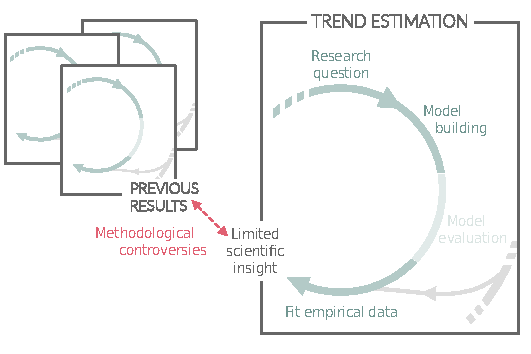
\includegraphics[width=\linewidth]{figures/trendestimation_details}

    % \vspace{-0.5cm}\captionsetup{font=footnotesize}\captionof{figure}{Caption}\label{fig:trends}
    \vspace*{1mm}
\end{minipage}

% Trends - outline current problem
%  Evidence of declining populations of vertebrate species in the 20th century gave rise a new subfield within ecology---conservation biology---now an entire discipline of its own that drives much of the policy-relevant science in ecology. 
% Evidence of declining populations of vertebrate species in the latter half of the 20th century, alongside increasing ecosystem health concerns, led to growing public concern about protecting and maintaining the environment, challenging ecology to help predict and prevent further losses \citep{soule1999conserving,soule1991conservation}. The idea that important taxa were declining was clear from data from certain species and their populations, such as elephants and rhinos \citep{soule1979benign,leader1990illegal}. 
% Such trends drove a number of new subfields within ecology---some of which are now complete disciplines within themselves \citep[such as conservation biology,][]{soule1985conservation}---focused on these problems, and potential ecological solutions to them CITES. Yet, as the magnitude and number of threats to these and other species have increased, with rates of habitat loss, overharvesting, pollution only increase, and anthropogenic climate change now clearly driving species loss \citep{waller2017bramble}, so has the data and its complexity. 
% Ecologists have now amassed data on populations and species over the globe, they have also engaged in an increasing number of debates on regional and global trends, with arguments over the magnitude and even direction \citep{Dornelas2014,Leung2020,terry2022no,muller2024weather}. 
In the current workflow for estimating trends over time a new model with a new estimate often leads to a paper (see Fig.) because ecologists spend far too little time interrogating their models with simulated data, or their model performance fit to empirical data. 
The Living Planet Index (LPI), which aims to include long-term data on vertebrate populations of species across the globe is emblematic of these conflicting results. With updated data released semi-annually (??) alongside new estimates of decline, a growing number of high-profile papers have challenged how strong the evidence is for population decline \citep{Dornelas2014,gonzalez2016estimating,wagner2021insect,muller2024weather}, with each paper taking a slightly different analytical approach. For example, \citet{Leung2020} published a mixture model that suggested most populations were not significantly declining, followed by other alternative modeling approaches \citep{Buschke2021,puurtinen2022living} including a recent one suggesting a basic analysis of the dataset should always include three sources of autocorrelation, finding trends that encompassed most previous results \citep{Johnson2024}. 

% Apparently conflicting results have made it harder for policy-makers to advance initiatives aimed at slowing declines, and has led to a debates within ecology about whether such analyses undermine public confidence in science  \citep{gonzalez2016estimating}. While shifting estimates are part of the process of science---refining our approaches and thus estimates over time---we argue much of the work underlying these debates stems from a poor workflow. 

% Functionally, research on the LPI has somewhat reverse-engineered the recommended workflow: after a series of papers debating different estimates from different models, more recent papers have focused on simulated data to highlight uncertainty given the model and data togethers \citep[though I don't think they link their simulations to the model they use that well,][]{dove2023quantifying,toszogyova2024mathematical}, but this should have been part of the process for the very first papers.
% While this debate captures part of the process of science---refining our approaches and thus estimates over time---it also makes it hard for policy-makers to do (?? something) and has led to a debates within ecology about whether such analyses undermine public confidence in science  (CITES Biodiversity debate). 
% \citet{Buschke2021} who focused on adding random population variation
\vfill

\columnbreak

\centerline{\bf Mechanistic forecasting}
\vspace*{2mm}
\begin{minipage}[t]{\linewidth}
    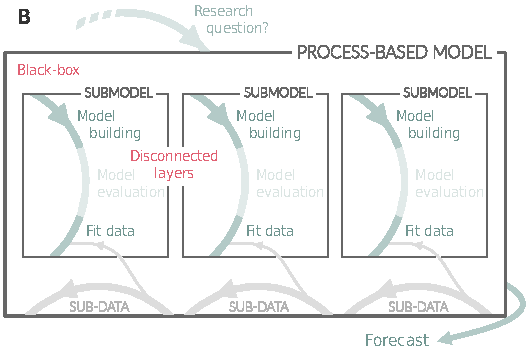
\includegraphics[width=\linewidth]{figures/forecasting_details}

    % \vspace{-0.5cm}\captionsetup{font=footnotesize}\captionof{figure}{Caption}\label{fig:trends}
    \vspace*{1mm}
\end{minipage}

\noindent % Process-based models are built on explicit mathematical equations to describe (supposedly causal) relationships between environmental drivers and ecological responses. 
% They also often incorporate empirical relationships, particularly when knowledge is incomplete or when some processes are intentionally omitted. Processes are often represented at different nested spatiotemporal scales, depending on the underlying assumptions. 
Model development is the central step of the process-based workflow, typically requiring several years, yet it often remains opaque from an external perspective. The step of designing the model---translating knowledge and hypotheses into mathematical equations and parameters---is often blurred with the step of model calibration (or tuning), where parameter values are inferred. Models are often treated as an accumulation of multiple submodels, each governing one or several ecological processes. Rather than being fitted as a whole, submodels are calibrated separately against specific subsets of data, and some parameters are simply prescribed (i.e. fix to a value found in the literature) or tuned to reproduce some observations or theory. The way models are currently calibrated is not a coincidence,
but rather an inappropriate way to accommodate their complexity, where many parameters compensate for one another.

\vfill

\end{multicols}}

\centerline{\bf Common solution!}
\vspace{0.2cm}
\noindent\makebox[\textwidth][c]{
\begin{minipage}{0.8\linewidth}
    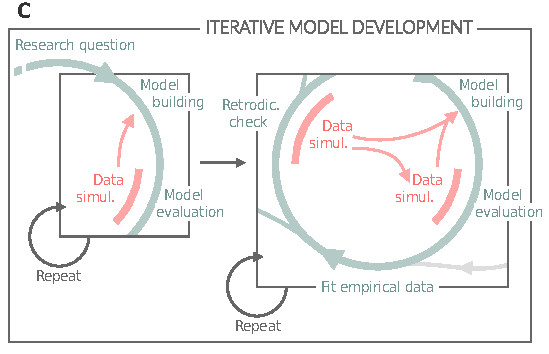
\includegraphics[width=\linewidth]{figures/iterativeworkflow_details}

    % \vspace{-0.5cm}\captionsetup{font=footnotesize}\captionof{figure}{Caption}\label{fig:trends}
    \vspace*{1mm}
\end{minipage}}

\end{tcolorbox}



\section{Barriers and opportunities}

We believe our workflow could help advance ecological science and its applications, but widespread use of it requires overcoming major hurdles that pervade science.  
One well-known hurdle is that the pressure to publish academic work, which can lower research standards and make the added effort of this workflow seem ill-placed. This may be especially true for those who see science rewarded mostly through the shear number of publications. But for those more focused on the long-term value of their work---for example, how well cited their papers are over a longer-time scale---we think this workflow can help. Further, growing concerns about how reproducible science is, especially in ecology where samples sizes are low and effects likely non-linear and complex, we believe adopting the workflow will pay off in the longer term, as more value is placed on research that carefully developed, openly shared (for data and code) and acknowledges its uncertainty towards the aim of improving future data collection and model development (see Fig). 

\subsection{Comprehensive training}
% emw03april: massively shorten?
Advancing ecology to where most researchers see models built more flexibly from their understanding of their ecological systems will not happen rapidly without a major shift in training, however. Much of ecology still divides the world into training for those focused on several groups. First, those who will conduct field and lab studies often learn a suite of particular tests matched to particular experiment designs or to simply match their predictor and response data to a flow diagram of variable types (add EXAMPLE and reference, something like: categorical $y$ and binary $y$ means ... I dunno, chi square?) and are left adrift later when asked to simulate any sort of simple model because they were never taught what a model fundamentally is. Instead, they are expected to collaborate with others when they need more complex models, which is a second group of ecological researchers---those who focus on complex statistical models and were thus trained more in model development, but often for highly specific applications (e.g., wildlife population estimates) where they may rarely build totally new generative models. Separate from these groups, process-based modelers do their own thing. 
% process-based modelers---often with a physical or ecophysiological background---mostly focus on simulating some mechanisms 
% hmm some people talk about simulation models (for process-based models), I agree but I'm afraid in would not be clear with the data simulation we try to highlight
Few of these groups have integrated data simulation into their statistical or scientific workflows, which is generally reserved as a form of training needed mainly by those specializing in theoretical ecology, who often solve analytical equations but rarely link to empirical data. While specialization is valuable, we argue the fundamental training in ecology has overly-siloed these groups and prevented more rapid progress.

Training all ecologists in our proposed workflow would break down barriers between different groups of ecologists today with likely major benefits for science. Instead of training some ecologists extensively in experimental design and tests that may match certain designs (though rarely do for ecological data, CITES), training in our workflow would focus on learning to generate questions and then models, and then to simulate data from them. This would mean training all ecologists to link the ecological processes they study with the mathematical models that may describe them. Through this and retrodictive checks most ecologists would more easily think through what parameters are most critical to their question and or aim (e.g., management) and also gain a much stronger connection to the level of uncertainty in many of ecological estimates. Empirical ecologists would be more likely to recognize critical gaps in current models fit by those specializing in ecological modeling and help advance those models. Process-based modelers may start a new generation of simpler models that are more tractable to theoretical ecologists, who may suddenly see bridges from their work to empirical data and forecasting. 
% Perhaps the only drawback would be to those focused on statistical models, whose gate-keeping would suddenly fail them and they would have to do more that just say how amazing they are... 
Those focused on learning complex statistical models may find many of the field now share their excitement and interest in more generative models, and could focus on adapting approaches to better forecasts or something.

% \subsection{Tractable models with mechanistic understanding as an alternative to machine learning} % not a good subheader title
\subsection{A tractable alternative to machine learning}

An universal workflow offers an opportunity to bridge statistical and process-based frameworks, integrating mechanistic knowledge and leveraging robust statistical approaches \citep[e.g.][]{rounce2020quantifying}. Process-based models would no longer be perceived as deterministic black boxes by other researchers but rather as robust statistical frameworks encapsulating both data structure and mechanistic knowledge. And it would also be an opportunity to spread the incorporation of mechanistic assumptions beyond the process-based modeling community.
In a world where machine learning is rapidly advancing, there is no point of sticking to traditional methods if no changes are made. Machine learning will likely surpass process-based models if the latter lack a robust estimation of their parameters and fall in a complexity trap, at the cost of their interpretability. Similarly, trend analysis, when the focus is on methodological controversies (due to the lack of an iterative workflow) rather than on a robust mechanistic foundation, offers no clear advantage over machine learning.

% emw03april: move this somewhere else?
Today model development in ecology is rarely transparent, which limits how easily the research community can understand modes, and thus identify potential issues. Instead of broad inclusive conversations about how to improve models to advance our ecological understanding, a significant portion of scientific debate today has become lost in methodological considerations, but we believe our workflow provides an tractable step to fixing this. By focusing on model development more tightly tied to ecological expertise, we ague this workflow should broader the community that contributes to model development. As ecologists are increasingly expanding their computational toolkits, many field, and lab and other forms of `empirical' ecologists have the basic tools to follow this workflow to build models that better represent their ecological, and---most importantly---to interrogate them.





% This type of workflow-focused training would make forecasting from models far more tractable ... 



%\item What are current workflows and where are they limiting us?
%\begin{enumerate}
%\item For trends ...
%\begin{enumerate}
%\item easy to find different trends through small model tweaks to analyses and/or different data
%\item For example, right now many different papers report different biodiversity trends (LPI example?)
%\item New workflow would make ecologists understand uncertainty in their model data/combo (and perhaps not see/publish results as so divergent?)
%\end{enumerate}
%\item For forecasting ... (somehow jump to our focus on process-based models PBMs here? Something like, forecasting is big and there are diverse methods! Near-term iterative, correlative niche models, but PBMs are often considered the gold standard ... mention machine learning?)
%\begin{enumerate}
%\item as many models as researchers working on process-based models 
%\item + accumulation of successive layers in the development of models = significant challenge to scientific transparency, reproducibility, interpretability\\
%models often draw inspiration from each other, which is good (way to do science), but not always explicit... (some issues: arbitrarily established parameter value in one model then transmitted to multiple models)
%\item focus of researchers: always integrate new mechanisms, new parameters, to increase "realism"...  they intuitively "feel" what kinds of adjustments is needed... but opaque from an external perspective ("black box" of model building and calibration)
%\item models rarely fitted as a whole, dozens of parameters without explicitly quantifying parameter uncertainty, and often neglect to propagate this uncertainty
%\item simulations of models themselves became a subject of study to disentangle all the processes modelled and understand model sensitivity 
%\end{enumerate}
%\end{enumerate}

%Miscellaneous notes/points without a home
%\begin{enumerate}
%\item Ecologists need to race the same data to make progress for trends and for forecasting (point to make at end of paper maybe? And what is the workflow for this?) ... though LPI is used a lot, perhaps it is  sign that ecology is ready to start racing the same data, but then we need `analysis-ready' data so we're not all slightly differently cleaning the data etc..
%\item Machine learning threatens utility of PBMs
%\item We need more uncertainty propagation for trends and forecasting (uncertainty is esp. ignored in PBMs)
%\item This workflow should lead to less model comparison (AIC, stepwise)
%\item This workflow works for machine learning!
%\item PBM: workflow should require estimating all parameters together; data simulation should reduce parameter number and highlight non-biol results
%\item Current trend workflow: Should be research question focused?
%\end{enumerate}
%
%Miscellaneous notes/points from thinking over 22-23 March weekend ...
%\begin{enumerate}
%\item Workflows emphasize there is no easy fix to better science or better stats
%\item Maybe do a retrodictive check example with LPI? Including showing how even the Freckleton work could do more? 
%\item What's the pathway from model comparison of many covariates to something else? Sometimes it seems like it's just prediction shoved into a mechanistic study, but if the goal is mechanism, there needs to be more work that either models these covariates together in a useful way (sort of approaching process-models!) or gets down to the fewer extremely relevant ones. 
%\item When do we need to open up the black box? Something about we need better training for what science is and our goals; machine learning is not often helping with advancing \emph{science}
%\item Scott Collins point that forecasting is not science (he claims a bunch of economists, weather folks etc. came to an ecological forecasting meeting and tried to explain that forecasting is an outcome of science, but it's not something you do science ON)
%\end{enumerate}

\clearpage
\bibliography{forecastflows}

\end{document}